\documentclass{article}

\usepackage{graphicx}
\usepackage{tikz}
\usepackage{tikzsymbols}
\usetikzlibrary{calc,patterns,shapes.geometric}
\pagestyle{empty}
\usepackage[margin=0pt]{geometry}
\geometry{papersize={14in,12in}}

\def\centerarc[#1](#2)(#3:#4:#5){\draw[#1] ($(#2)+({#5*cos(#3)},{#5*sin(#3)})$) arc (#3:#4:#5);}

\begin{document}
	\begin{figure}
		\centering
		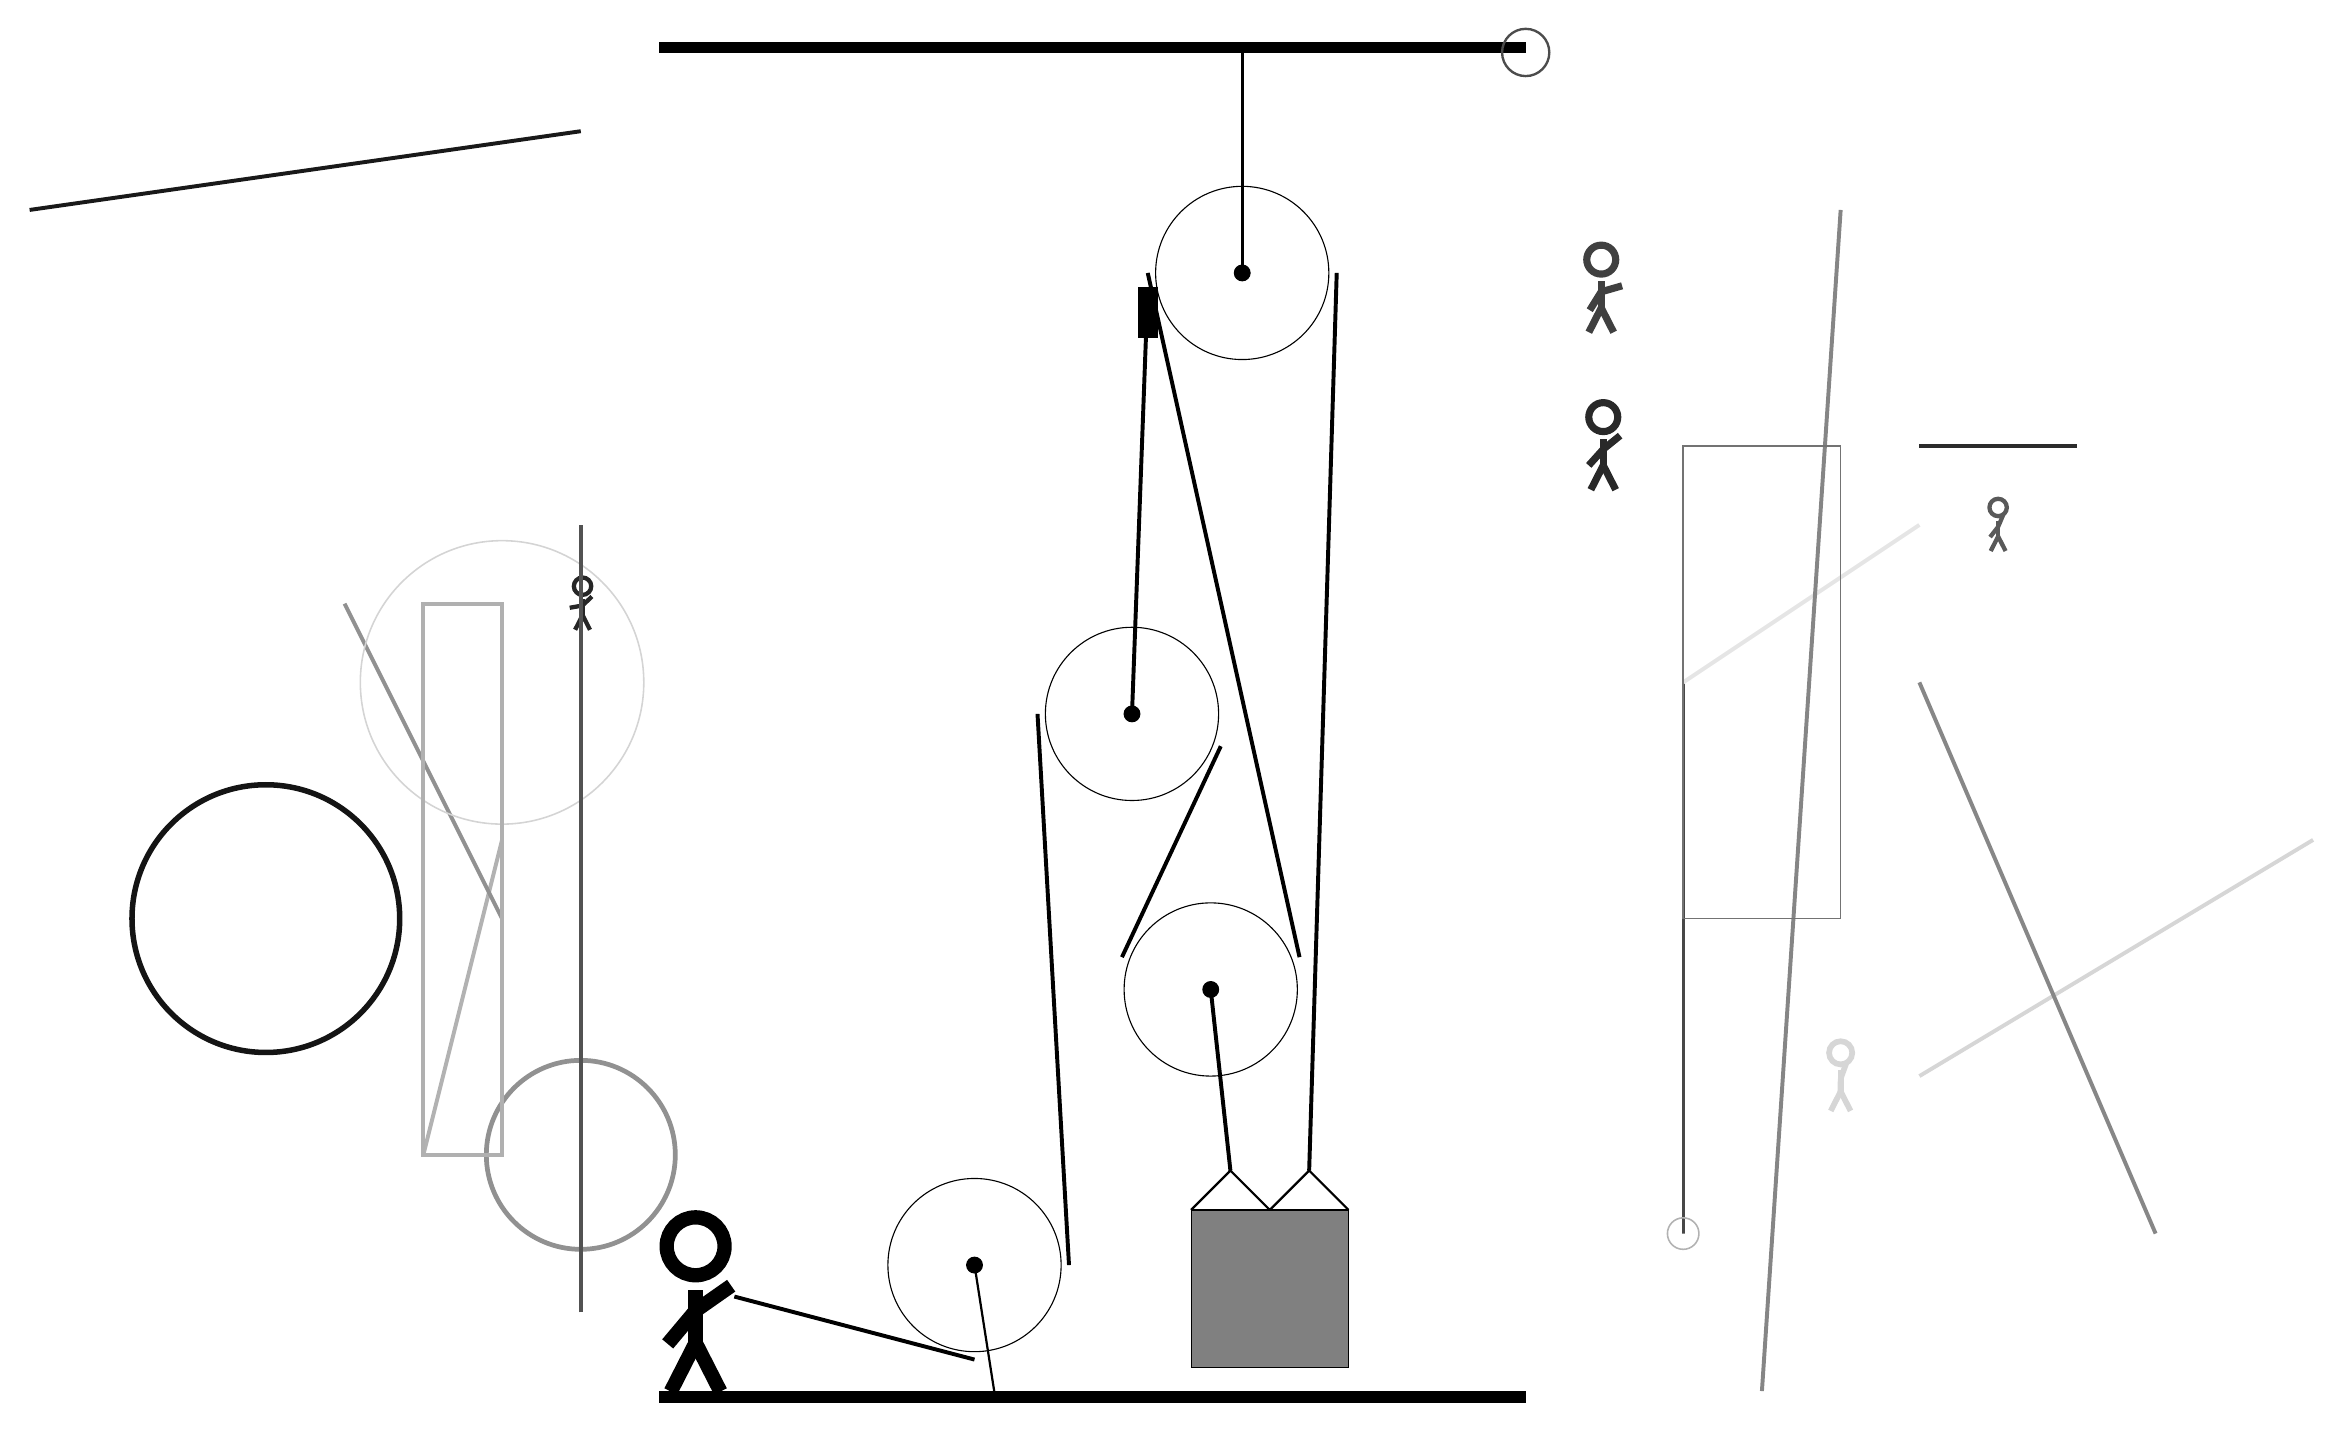
\begin{tikzpicture}
			%%%%% START %%%%%
			
			\draw[fill=black] (-6, 14) rectangle (5, 14.125);
			
			\draw (0, 5.6) circle (1.1);
			\draw[fill=black] (0, 5.6) circle (0.1);
			
			\draw (1, 2.1) circle (1.1);
			\draw[fill=black] (1, 2.1) circle (0.1);
			
			\draw (1.4, 11.2) circle (1.1);
			\draw[fill=black] (1.4, 11.2) circle (0.1);
			\draw[very thick] (1.4, 11.2) -- (1.4, 14);
			
			\draw (-2, -1.4) circle (1.1);
			\draw[fill=black] (-2, -1.4) circle (0.1);
			\draw[thick] (-2, -1.4) -- (-1.75, -3);
			
			
			\draw[thick]  (0.75, -0.7) -- (1.25, -0.2) -- (1.75, -0.7) -- (2.25, -0.2) -- (2.75, -0.7);
			\draw[fill=black!50] (0.75, -0.7) rectangle (2.75, -2.7);
			\draw[line width=0.5mm] (-5.05, -1.8) -- (-2, -2.6);
			\centerarc[line width=0.5mm](-2, -1.4)(270:360:1.2000000000000002);
			\draw[line width=0.5mm] (-0.8, -1.4) -- (-1.2, 5.6);
			\draw[line width=0.5mm] (0, 5.6) -- (0.2, 11.0);
			\draw[line width=0.5mm, fill=black](0.1, 10.4) rectangle (0.3, 11.0);
			\centerarc[line width=0.5mm](0, 5.6)(-20:180:1.2000000000000002);
			\draw[line width=0.5mm] (1.1276, 5.1896) -- (-0.1276, 2.5104);
			\centerarc[line width=0.5mm](1, 2.1)(160:380:1.2000000000000002);
			\draw[line width=0.5mm] (2.1276, 2.5104) -- (0.2, 11.2);
			\draw[line width=0.5mm](1, 2.1) -- (1.25, -0.2);
			\centerarc[line width=0.5mm](1.4, 11.2)(0:180:1.2000000000000002);
			\draw[line width=0.5mm] (2.6, 11.2) -- (2.25, -0.2);
			
			\node[line width=0.2mm, color=black!16] at (9, 1) {\Strichmaxerl[4][89][70]};
			
			\node[line width=0.3mm, color=black!84] at (6, 9) {\Strichmaxerl[5][48][39]};
			\node[line width=0.5mm, color=black!65] at (11, 8) {\Strichmaxerl[3][52][67]};
			\draw[line width=0.5mm, color=black!30](-8, 4) -- (-9, 0);
			
			\draw [line width=0.3mm, color=black!70](5, 14) circle (0.3);
			
			\node[line width=0.7mm, color=black!85] at (-7, 7) {\Strichmaxerl[3][10][44]};
			\draw [line width=0.6mm, color=black!43](-7, 0) circle (1.2);
			\draw[line width=0.5mm, color=black!43](-8, 3) -- (-10, 7);
			\node[line width=0.3mm, color=black!75] at (6, 11) {\Strichmaxerl[5][58][16]};
			\draw [line width=0.2mm, color=black!17](-8, 6) circle (1.8);
			\draw[line width=0.5mm, color=black!16](10, 1) -- (15, 4);
			\draw[line width=0.4mm, color=black!72] (7, -1) rectangle (7, 6);
			\draw[line width=0.5mm, color=black!90](-7, 13) -- (-14, 12);
			\draw[line width=0.5mm, color=black!83](10, 9) -- (12, 9);
			\draw [line width=0.7mm, color=black!92](-11, 3) circle (1.7);
			\draw[line width=0.5mm, color=black!10](7, 6) -- (10, 8);
			
			\draw[line width=0.5mm, color=black!31] (-8, 0) rectangle (-9, 7);
			\draw[line width=0.5mm, color=black!48](9, 12) -- (8, -3);
			\draw[line width=0.2mm, color=black!55] (7, 3) rectangle (9, 9);
			\draw [line width=0.2mm, color=black!30](7, -1) circle (0.2);
			\draw[line width=0.5mm, color=black!47](10, 6) -- (13, -1);
			
			\draw[line width=0.5mm, color=black!68](-7, -2) -- (-7, 8);
			
			
			\node at (-5.5, -1.9) {\Strichmaxerl[10][50][35]};
			
			\draw[fill=black] (-6, -3) rectangle (5, -3.15);
			
			%%%%% END %%%%%
		\end{tikzpicture}
	\end{figure}	
\end{document}